% Created 2018-12-17 lun 14:29
% Intended LaTeX compiler: pdflatex
\documentclass[xcolor={usenames,svgnames,dvipsnames}]{beamer}
\usepackage[utf8]{inputenc}
\usepackage[T1]{fontenc}
\usepackage{graphicx}
\usepackage{grffile}
\usepackage{longtable}
\usepackage{wrapfig}
\usepackage{rotating}
\usepackage[normalem]{ulem}
\usepackage{amsmath}
\usepackage{textcomp}
\usepackage{amssymb}
\usepackage{capt-of}
\usepackage{hyperref}
\usepackage{color}
\usepackage{listings}
\usepackage{mathpazo}
\usepackage{gensymb}
\usepackage{amsmath}
\usepackage{chemarr}%flechas para reacciones químicas (SFER.tex)
\bibliographystyle{plain}
\AtBeginSubsection[]{\begin{frame}[plain]\tableofcontents[currentsubsection,sectionstyle=show/shaded,subsectionstyle=show/shaded/hide]\end{frame}}
\AtBeginSection[]{\begin{frame}[plain]\tableofcontents[currentsection,hideallsubsections]\end{frame}}
\usepackage[emulate=units]{siunitx}
\sisetup{fraction=nice, decimalsymbol=comma, retain-unity-mantissa = false}
\newunit{\wattpeak}{Wp}
\newunit{\watthour}{Wh}
\newunit{\amperehour}{Ah}
\usepackage{steinmetz}
\hypersetup{colorlinks=true, linkcolor=Blue, urlcolor=Blue}
\renewcommand{\thefootnote}{\fnsymbol{footnote}}
\beamertemplatenavigationsymbolsempty
\setbeamertemplate{footline}[frame number]
\setbeamercolor{alerted text}{fg=blue!50!black} \setbeamerfont{alerted text}{series=\bfseries}
\usetheme[hideothersubsections]{Goettingen}
\usecolortheme{rose}
\usefonttheme{serif}
\author{Oscar Perpiñán Lamigueiro}
\date{\url{http://oscarperpinan.github.io}}
\title{Sistemas Fotovoltaicos de Bombeo}
\subtitle{Diseño}
\hypersetup{
 pdfauthor={Oscar Perpiñán Lamigueiro},
 pdftitle={Sistemas Fotovoltaicos de Bombeo},
 pdfkeywords={},
 pdfsubject={},
 pdfcreator={Emacs 25.2.2 (Org mode 9.1.13)}, 
 pdflang={Spanish}}
\begin{document}

\maketitle

\begin{frame}[label={sec:orged00caf}]{}
\begin{center}
\begin{center}
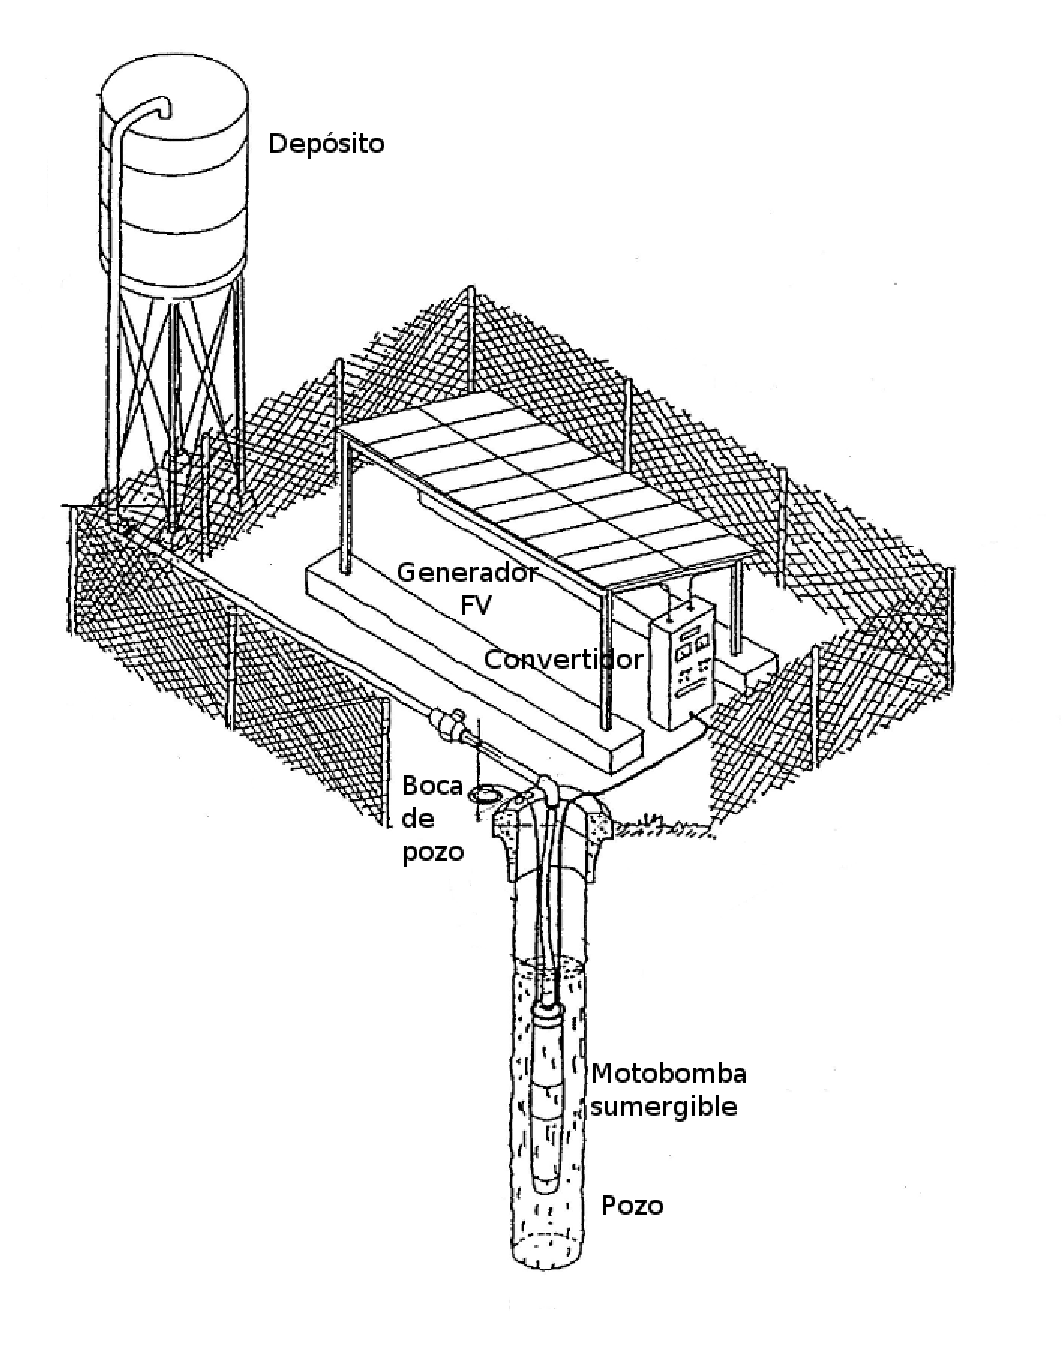
\includegraphics[height=0.9\textheight]{../figs/EsquemaBombeo_oscar.pdf}
\end{center}
\end{center}
\end{frame}


\section{Caudal}
\label{sec:orge253c9b}


\begin{frame}[label={sec:orgb97c54d}]{Necesidades de caudal}
\begin{block}{Valores de referencia}
\begin{itemize}
\item \alert{OMS}: 50 litros diarios por habitante.

\item En \alert{crisis humanitarias}, mínimo 3 litros diarios en climas templados y 5 litros en climas cálidos.

\item En \alert{programas de cooperación}, 30 a 35 litros diarios por persona.

\item Para \alert{sistemas fotovoltaicos}, se recomienda 25 litros diarios por habitante (fuentes comunitarias) o 45 litros (con grifo en cada domicilio).

\item \alert{Contexto}: en grandes ciudades 250 litros diarios por habitante.
\end{itemize}
\end{block}
\end{frame}


\begin{frame}[label={sec:org4f83ca2}]{Potencia hidráulica}
\begin{itemize}
\item La \alert{potencia hidráulica}, \(P_{H}\), necesaria para bombear agua es una función de,

\begin{itemize}
\item La \alert{altura vertical aparente}, \(H_{v}\)

\item El \alert{caudal de agua}, \(Q\)
\end{itemize}
\end{itemize}

$$P_{H}=g\cdot\rho\cdot Q\cdot H_{v}$$

\begin{itemize}
\item Cambiando las unidades (\(P_{H}\) en watios, \(H_{v}\) en metros y \(Q\) en \(\si{\meter\cubed\per\hour})\):
\end{itemize}
\[
P_{H}=2.725\cdot Q\cdot H_{V}
\]
\end{frame}

\begin{frame}[label={sec:org976e952}]{Potencia eléctrica de la motobomba}
\begin{itemize}
\item La \alert{potencia de salida de la bomba} incluye las \alert{perdidas de fricción en la tubería}, \(P_{mp} = P_{H} + P_{f}\).

\item Se puede asimilar a una altura equivalente \(H_{T} = H_{v}+H_{f}\):
\end{itemize}

\[
P_{mp}=2.725\cdot Q\cdot H_{T}
\]

\begin{itemize}
\item Con la eficiencia de la motobomba obtenemos la \alert{potencia eléctrica a la entrada de la motobomba}:
\end{itemize}
\[
  P_{el}=\frac{P_{mp}}{\eta_{mp}} = \frac{2.725\cdot Q\cdot H_{T}}{\eta_{mp}}
\]
\end{frame}


\begin{frame}[label={sec:org798f7f5}]{Potencia eléctrica del generador}
Esta potencia eléctrica requerida por la motobomba es entregada por un generador FV y un acondicionador de potencia

\[
  P_{el}=\frac{G}{G^{*}} \cdot P_{g}^{*} \cdot \frac{\eta_{g}}{\eta_{g}^{*}} \cdot \eta_{inv}
\]

Por tanto,

\[
  \frac{2.725\cdot Q\cdot H_T}{\eta_{mp}} \simeq  \frac{G}{G^{*}} \cdot P_{g}^{*} \cdot \frac{\eta_{g}}{\eta_{g}^{*}}  \cdot \eta_{inv}
  \]
\end{frame}



\begin{frame}[label={sec:orgd4fbe67}]{Caudal diario}
\[
  \frac{2.725\cdot Q\cdot H_T}{\eta_{mp}} \simeq  \frac{G}{G^{*}} \cdot P_{g}^{*} \cdot \frac{\eta_{g}}{\eta_{g}^{*}}  \cdot \eta_{inv}
  \]

\begin{itemize}
\item El \alert{caudal diario} bombeado por este conjunto es:
\end{itemize}
\[
  Q_{d}=\intop_{d}\frac{\frac{G}{G^{*}} \cdot P_{g}^{*} \cdot \frac{\eta_{g}}{\eta_{g}^{*}}  \cdot \eta_{inv} \cdot \eta_{mp}}{2.725\cdot H_{T}}\mathrm{dt} 
\]


\begin{itemize}
\item \alert{Todos los parámetros varían a lo largo del tiempo} (variaciones de la temperatura ambiente y de la irradiancia; comportamiento dinámico de los pozos)

\item Integral no resoluble salvo por métodos numéricos (simulación).
\end{itemize}
\end{frame}

\section{Altura}
\label{sec:orgcc08820}

\begin{frame}[label={sec:orge564e87}]{Altura total equivalente}
$$Q_{d}=\intop_{d}\frac{P_{g}^{*}\cdot\frac{G}{G^{*}}\frac{\eta_{g}}{\eta_{g}^{*}}\cdot\eta_{inv}\cdot\eta_{mp}}{2.725\cdot H_{T}}\mathrm{dt}$$


\begin{itemize}
\item Definimos una \alert{altura total equivalente}, \(H_{TE}\), con las siguientes suposiciones:

\begin{itemize}
\item Las \alert{pérdidas de fricción en tubería son despreciables} (\(H_{f}<0.05\cdot H_{T}\)).

\item El \alert{nivel del agua dentro del pozo se mantiene constante}
\end{itemize}
\end{itemize}

\[
Q_{d}=\frac{P_{g}^{*}}{2.725\cdot G^{*}\cdot H_{TE}}\cdot\intop_{dia}G\cdot\frac{\eta_{g}}{\eta_{g}^{*}}\cdot\eta_{inv}\cdot\eta_{mp}\mathrm{dt}
\]

\begin{itemize}
\item Ahora el cálculo en la integral sólo \alert{depende de la radiación, temperatura, y equipos}.
\end{itemize}
\end{frame}


\begin{frame}[label={sec:orgded4b99}]{Caracterización de pozos}
\begin{itemize}
\item Supongamos que el pozo está caracterizado con tres parámetros:

\begin{itemize}
\item \alert{Nivel estático}, \(H_{st}\)

\item \alert{Nivel dinámico}, \(H_{dt}\)

\item \alert{Caudal de ensayo}, \(Q_{t}\).
\end{itemize}

\item Deseable realizar \alert{ensayo de bombeo para caracterizar los pozos} con bomba portátil empleando el \alert{caudal máximo del pozo}, \(Q_{max}\) (por tanto, supondremos \(Q_t = Q_{max}\))
\end{itemize}
\end{frame}

\begin{frame}[label={sec:org9bc71f4}]{Altura total equivalente}
Calculamos la \alert{altura total equivalente} con:

\[
\boxed{H_{TE}=H_{ot} + H_{st} + (\frac{H_{dt} - H_{st}}{Q_{T}}) \cdot Q_{AP} + H_{f}(Q_{AP})}
\]

\begin{itemize}
\item \(H_{OT}\),  altura desde la salida de agua hasta el suelo.

\item Nivel estático, \(H_{st}\)

\item Nivel dinámico, \(H_{dt}\)

\item Caudal aparente: \(Q_{AP} = \alpha \cdot Q_{d}\) (\(\alpha= 1/24 = 0.0416\, h^{-1}\)).

\item \(H_{f}(Q_{AP})\), pérdidas en la tubería al caudal aparente.
\end{itemize}
\end{frame}

\section{Potencia del generador}
\label{sec:orgaff3009}
\begin{frame}[label={sec:org727a1b5}]{Formula aproximada}
\begin{itemize}
\item Punto de partida
\end{itemize}
$$Q_{d}=\frac{P_{g}^{*}}{2.725\cdot G^{*}\cdot H_{TE}}\cdot\intop_{dia}G\cdot\frac{\eta_{g}}{\eta_{g}^{*}}\cdot\eta_{inv}\cdot\eta_{mp}\mathrm{dt}$$

\begin{itemize}
\item Consideramos constantes las eficiencias
\begin{itemize}
\item \(\dfrac{\eta_{g}}{\eta_{g}^{*}}=0.85\)
\item \(\eta_{mp}=0.35\)
\item \(\eta_{inv}=0.9\)
\end{itemize}
\end{itemize}
\begin{block}{Potencia del Generador}
\[
\boxed{P_{g}^{*}=\frac{10\cdot H_{TE}\cdot Q_{d}}{G_{d}/G^{*}}}
\]
\end{block}
\end{frame}

\begin{frame}[label={sec:orgde4b524}]{}
\begin{block}{Ejemplo}
Calcula la potencia de un generador FV para bombear un caudal diario de \(\SI{30}{\meter\cubed\per\Day}\) a \(H_{TE}=\SI{40}{\meter}\) en un lugar de radiación diaria media \(G_{d}=\SI{5}{\kilo\watt\hour\per\meter\squared\per\Day}\).
\end{block}
\end{frame}


\section{Procedimiento de diseño}
\label{sec:orge339969}

\begin{frame}[label={sec:orgc30d28c}]{Elección de la bomba}
\begin{enumerate}
\item A partir del caudal diario requerido y la altura total equivalente, se calcula la potencia aproximada del generador FV.

\item Dividiendo el caudal diario requerido por la radiación diaria media, se obtiene un \emph{caudal instantáneo medio}.

\item Con este caudal, se acude al catálogo del fabricante (\emph{por ejemplo, la nomenclatura de Grundfos para las bombas sumergibles es SP-XX-YY, siendo XX el caudal instantáneo nominal de la bomba}) y se elige un grupo de bombas en el entorno.
\end{enumerate}
\end{frame}

\begin{frame}[label={sec:org3f3b55d}]{Curvas HQ}
\begin{columns}
\begin{column}{0.5\columnwidth}
\begin{center}
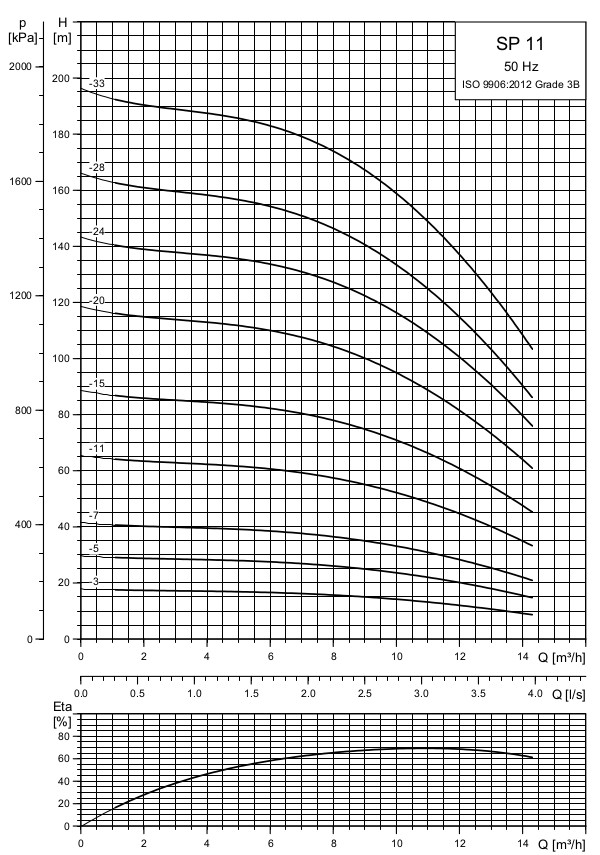
\includegraphics[height=0.8\textheight]{../figs/CurvaSP11.jpg}
\end{center}
\end{column}

\begin{column}{0.5\columnwidth}
\begin{itemize}
\item Los catálogos recogen información del \alert{funcionamiento instantáneo a frecuencia nominal}.
\item Las curvas H-Q \alert{no} son de uso inmediato para el dimensionado de un SFB.
\end{itemize}
\end{column}
\end{columns}
\end{frame}


\begin{frame}[label={sec:orgd66ddf2}]{Curvas HQ a frecuencia variable}
\begin{itemize}
\item Para aproximar el funcionamiento en frecuencia variable, es recomendable \alert{multiplicar el valor de \(H_{TE}\) por un factor de \(1.4\)}.

\item Leyes de la semejanza (rendimiento constante)
\end{itemize}

\begin{align*}
Q &\propto n &H &\propto n^{2}\\
P_{mec} &\propto n^{3} &T &\propto n^{2}
\end{align*}

\begin{center}
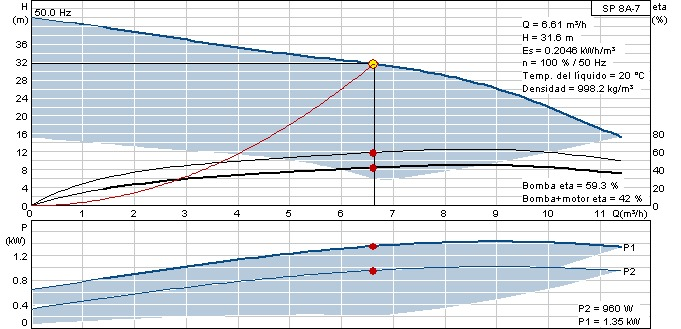
\includegraphics[width=.9\linewidth]{/home/oscar/github/esf/figs/CurvaHQ.png}
\end{center}
\end{frame}



\begin{frame}[label={sec:org942efed}]{Simulación}
\begin{itemize}
\item Es recomendable simular el funcionamiento del sistema para afinar el dimensionado.
\item El resultado es un gráfico de doble entrada para un modelo concreto de bomba
\end{itemize}
\begin{center}
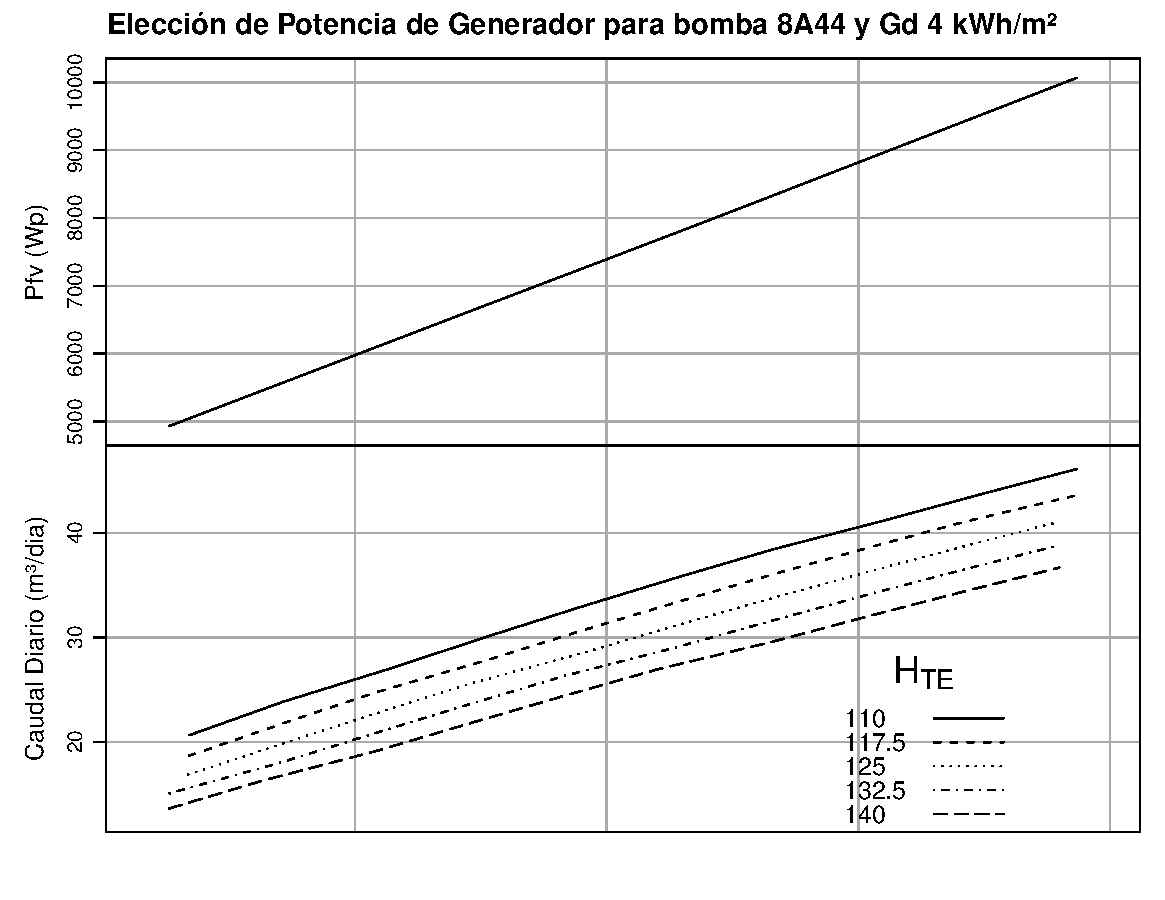
\includegraphics[width=.9\linewidth]{../figs/AbacoBomba.pdf}
\end{center}
\end{frame}

\begin{frame}[label={sec:org2b20627}]{Configuración eléctrica}
\begin{itemize}
\item La \alert{tensión de entrada al variador} debe ser:$$V_{DC}=\frac{\sqrt{2}V_{AC}}{1.1}$$

\item Ejemplo: para una bomba de tensión de \(230\, V_{ac}\) se necesita una tensión en la entrada que no sea inferior a \(\simeq300\, V_{dc}\).

\item A partir de esta tensión se configura el \alert{número de módulos por serie} y el \alert{número de ramas} del generador.
\end{itemize}
\end{frame}

\begin{frame}[label={sec:org43c3673}]{Pozo, Depósito y Tubería}
\begin{block}{Caudal máximo del pozo}
Como seguridad, se debe comprobar que cuando la potencia entregada por el generador es igual al 80\% de su potencia nominal, el caudal bombeado correspondiente no excede el máximo admisible por el pozo.
\end{block}

\begin{block}{Tamaño del depósito}
El suficiente para \alert{1 o 2 días de consumo}
\end{block}

\begin{block}{Tubería}
A partir del caudal \(Q_{AP}\) y de la longitud de tubería necesaria, se elige el \alert{diámetro} de la misma (en curvas del fabricante) de forma que las pérdidas sean inferiores a un porcentaje prefijado de \(H_{TE}\).
\end{block}
\end{frame}
\end{document}